\renewcommand{\lastmod}{10. Oktober 2024}
\renewcommand{\chapterauthors}{Markus Lippitz}

\chapter{Wellenfunktionen}




% 3. Probability and Randomness and Wave particle duality
% Sim: Quantum Wave Interference
% • When we ask how students visualize light, ~40% have “Bohmian” view of particle traveling
% alongside EM wave.
% • We use sim to demonstrate how the double slit experiment shows that light must be both a
% wave that goes through both slits and a particle that hits the screen at a single location. This
% lecture led to an unexpected onslaught of deep, fundamental questions that took up nearly an
% entire class period. Many students ask whether the particle is actually inside wave with a
% definition location that we just don’t know. Students get pretty frustrated with this class.


% 9. Double slit and Davisson Germer experiment
% Sims: Quantum Wave Interference, Davisson Germer: Electron Diffraction
% • Students have a much harder time thinking of electrons as waves than photons, because
% electrons have mass.
% • Students often think that the size of the wave packet, rather than the wavelength, should
% determine the spacing of the interference pattern.
% • We have noticed that students often miss the point of the Davisson Germer experiment. They
% remember that electrons were only detected at certain angles, but cannot explain why. They
% view the electrons as particles that happen to bounce off at certain angles for some reason
% they can’t understand, rather than recognizing how the observations can be explained by the
% wave nature of electrons. We have found two things that really help to address this:
% - Start with a review of the double slit experiment, a context where students understand
% interference much better, talking about how you would like to do this to test deBroglie’s
% hypothesis, and then explain why this is really hard to do and then talk about how the
% Davisson Germer experiment is analogous.
% - Use the Davisson Germer sim to illustrate how wave interference leads to peaks in
% intensity at certain angles.

% 10. Wave functions and probability
% • When we first introduce wave functions with arbitrary functions, students often don’t
% recognize these as waves because they think “waves” are sine waves.
% • “Wave number” is usually new and unfamiliar to students, and it’s worth spending 5 minutes
% to discuss why we define this quantity and how it relates to wavelength.

% 11. Wave packets and uncertainty principle
% Sims: Quantum Wave Interference, Quantum Tunneling, Fourier: Making Waves
% • We introduce wave packets early because they are much more intuitive than plane waves and
% easier to relate to “particles.”



\section{Überblick}

In diesem und im nächsten Kapitel werden wir uns mit den Grundlagen der Quantenmechanik beschäftigen. Die Quantenmechanik ist eine Theorie, die manchmal etwas unanschaulich ist, manchmal eher einem Kochrezept ähnelt, aber erstaunlich gut funktioniert. Die größte ungeklärte Frage ist derzeit wohl, wie sich die Quantenmechanik mit der Allgemeinen Relativitätstheorie vereinbaren lässt. Aber das braucht uns hier nicht zu interessieren. Die Quantenmechanik beschreibt Objekte durch eine \emph{Wellenfunktion}, die wir in diesem Kapitel einführen. Im nächsten Kapitel geht es um die \emph{Schrödingergleichung}, mit der man Wellenfunktionen findet.  Wenn Sie schon einmal eine Vorlesung über Quantenmechanik gehört haben, wird Ihnen vieles bekannt vorkommen. Im Rest der Vorlesung werden wir die Quantenmechanik benutzen, um Atome und Moleküle zu beschreiben.

Wir beginnen wieder mit dem Doppelspaltexperiment, da hier die Wellenfunktion der Photonen mit dem bereits bekannten elektrischen Feld verwandt ist. Wir werden sehen, dass wir nur Wahrscheinlichkeitsaussagen machen können. Das ist vergleichbar mit der Messunsicherheit, aber es ist eine fundamentale Eigenschaft der Theorie, die technisch nicht eliminiert werden kann. Sie ist so fundamental, dass mit der Heisenbergschen Unschärferelation sogar ein Zusammenhang zwischen den Unsicherheiten zweier komplementärer Größen besteht. Schließlich beschreiben wir Wellenpakete, die ein Modell für ein Teilchen im Wellenbild sein können.

Die Gliederung folgt wiederum  Kapitel 39 von \cite{Knight_physics}. Weiterhin finden sich gute andere Darstellungen in \cite{Haliday_Resnick}, \cite{Demtröder_ep3} und \cite{Haken_wolf_I}.


%Ich kann das Konzept einer Materiewelle benutzen um Experimente mit Teilchen zu erklären, insbesondere deren statistischen Aspekte.


\section{Das Doppelspaltexperiment mit Lichtwellen}

Kommen wir noch einmal auf das Doppelspaltexperiment von Young zurück, das Sie bereits in der Optik behandelt haben. Wir behandeln Licht als Welle und nicht als Teilchen. Eine ebene Welle fällt auf zwei (sehr dünne) Spalten in einem ansonsten undurchlässigen Schirm. Man kann sich vorstellen, dass von jedem Punkt in den Spalten eine Huygenssche Elementarwelle $E_{1,2}$ ausgeht, die man schreiben kann als 
\begin{equation}
    E_{i} = a_i \, \sin ( k \, r_i - \omega t) \quad \text{mit} \quad i = 1,2
\end{equation}
mit der Amplitude $a$ und dem Abstand $r$ vom Spalt. $k = 2 \pi / \lambda $ ist die Länge des Wellenvektors, auch Wellenzahl genannt.
Die Kreisfrequenz ist $\omega = c k$.


\begin{marginfigure}
    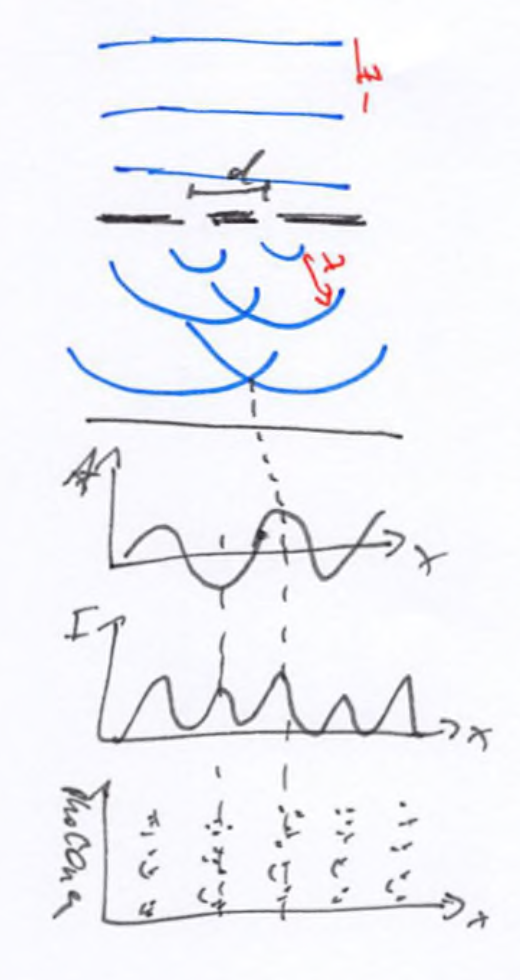
\includegraphics[width=\textwidth]{\currfiledir sketch/doubleslit.png}
    \caption{Beugung am Doppelspalt. Die Amplitude $A(x)$ am Schirm bestimmt die Intensität $I$ und die Wahrscheinlichkeit, Photonen am Ort $x$ zu detektieren.}
    \label{fig:3_Doppelspalt}
\end{marginfigure}


Auf dem Schirm überlagern sich die Wellen. Das Superpositionsprinzip besagt, dass das resultierende elektromagnetische Feld genau die Summe der beiden Felder ist, also $E = E_1 + E_2$. In der Optik haben Sie gesehen, dass sich daraus die folgende Amplitude $A(x)$ am Ort $x$ des Schirms ergibt
\begin{equation}
    A(x) = 2 a\cos \left( \frac{\pi d}{\lambda L} \, x \right)
\end{equation}
mit dem Abstand $L$ zwischen Spaltebene und Schirm und dem Abstand $d$ zwischen den beiden Spalten.\sidenote{Oben haben wir angenommen, dass die Spalten sehr dünn sind. Daher geht die Spaltweite nicht ein und die Gleichung wird einfacher.} Die Amplitude $A$ ist maximal ($A = 2a$), wenn sich zwei Wellenberge am Schrim treffen, und minimal ($A = -2 a$), wenn sich zwei Täler treffen.  Dazwischen gibt es Nulldurchgänge. 

Im Experiment wird nicht die Amplitude der Wellen beobachtet, sondern ihre Intensität $I \propto A^2$, d.h.
\begin{equation}
    I(x) = C \, \cos^2 \left( \frac{\pi d}{\lambda L} \, x \right)
\end{equation}
mit einer Proportionalitätskonstanten $C$. Die Nulldurchgänge der Amplitude ergeben somit ein Minimum der Intensität (destruktive Interferenz). Die Maxima der Amplitude ergeben unabhängig vom Vorzeichen ein Maximum der Intensität (konstruktive Interferenz). Nur die Intensität beschreibt also die experimentell beobachtbare Realität.


\section{Wahrscheinlichkeit}

\begin{marginfigure}
    \inputtikz{\currfiledir dart}
    \caption{Ergebniss der Dart-Würfe}
    \label{fig:3_dart}
\end{marginfigure}


Bevor wir zur Beschreibung durch Photonen kommen, müssen wir kurz über Wahrscheinlichkeiten sprechen. In einem Gedankenexperiment werfen Sie mit verbundenen Augen Dartpfeile auf eine Wand. Jeder Pfeil trifft die Wand, aber nicht immer an der gleichen Stelle. Nach 100 Würfen ergibt sich ein Muster wie in Abbildung  \ref{fig:3_dart}. Wo wird der nächste Wurf treffen? Das können wir nicht mit Sicherheit sagen. Aber wir können eine Wahrscheinlichkeit angeben. Bisher sind $N_A =45$ von $N = 100$ Würfen im Bereich A gelandet. Ob von den nächsten 100 Würfen wieder genau 45 Würfe hier landen, ist eher unwahrscheinlich. 100 Würfe sind einfach zu wenig. Deshalb definiert man die Wahrscheinlichkeit $P_A$ als Grenzwert für sehr viele Versuche:
\begin{equation}
    P_A =  \lim_{N \rightarrow \infty} \frac{N_A}{N} \quad .
\end{equation}
Für Abbildung \ref{fig:3_dart} können wir also nur $P_A \approx 0.45$ schreiben. 


Die Wahrscheinlichkeiten für sich ausschließende Ergebnisse addieren sich. Die Wahrscheinlichkeit, im Bereich A oder B zu landen, beträgt also
\begin{equation}
    P_{A oder B} = \lim_{N \rightarrow \infty} \frac{N_A + N_B}{N} = P_A + P_B
\end{equation}
und die Summe aller Wahrscheinlichkeiten ist eins, also 
\begin{equation}
    P_A + P_B + P_C = 1 \quad .
\end{equation}

Der erwartete Wert $N_{erw}$ für die Anzahl der Treffer im Bereich A ergibt sich durch Umformung zu 
\begin{equation}
    N_{A, erw} = P_A \, N \quad .
\end{equation}
Unsere beste Vorhersage für die Anzahl der Treffer nach 60 Versuchen ist also $0.45 \cdot 60 = 27 $. Die tatsächlich beobachtete Anzahl der Treffer kann davon abweichen. Je mehr Versuche $N$ durchgeführt werden, desto geringer wird die Abweichung sein.



\section{Interpretation des Interferenzmusters von Photonen }

Im letzten Kapitel haben wir bereits gesehen, welches Punktmuster Photonen auf einem Schirm hinter einem Doppelspalt hinterlassen (siehe Abb.~\ref{fig:3_Doppelspalt}). Dieses wollen wir nun etwas genauer betrachten. Wie ein Foto in der Zeitung besteht das Bild auf dem Schirm aus vielen Punkten, die mehr oder weniger dicht beieinander liegen. Und wie bei den Dartpfeilen können wir nicht sagen, wo das nächste Photon detektiert wird. Aber es gibt Regionen, in denen dies mehr oder weniger wahrscheinlich ist.

Wir definieren entlang der Ortskoordinaten $x$ einen schmalen Streifen der Breite $\delta x$ und Höhe $H$ und zählen alle Photonen, die in diesen Streifen gefallen sind. Diese Zahl nennen wir hier $N(x, \delta x)$. Sie hängt natürlich von der Position $x$ ab, ob es sich um eine hellere oder dunklere Stelle des Sinterferenzmusters handelt. Wir definieren die Wahrscheinlichkeit $WK$ wieder als Grenzwert für eine Gesamtzahl von Photonen $N$
\begin{equation}
    WK(x, \delta x) = \lim_{N \rightarrow \infty} \, \frac{N(x, \delta x)}{N} \quad .
\end{equation}
Von einer guten Theorie erwarten wir, dass sie diese Wahrscheinlichkeit $WK(x, \delta x)$ vorhersagt, so dass wir die erwartete Anzahl von Photonen in diesem Intervall berechnen können, d.h. 
\begin{equation}
    N(x, \delta x)_{ erw} = WK(x, \delta x) \, N \quad .
\end{equation}
Wir werden nicht in der Lage sein, den Auftreffpunkt des nächsten Photons vorherzusagen. Aber wir werden in der Lage sein, die Wahrscheinlichkeit und damit die Anzahl der zu erwartenden Photonen in einem schmalen Streifen zu berechnen.


\section{Photonen- und Wellenbild vereinigen}

Wie erhält man die Wahrscheinlichkeit $WK(x, \delta x)$? Hier hilft uns die Energie des Lichts auf dem Schirm. Die Energie, die in dem Streifen mit der Breite $\delta x$ und der Höhe $H$ an der Position $x$ einfällt, sei $E(x, \delta x)$. Für sie gilt 
\begin{equation}
    E(x, \delta x) = I(x) \, \delta x \, H
\end{equation}
wobei angenommen wird, dass $\delta x$ so klein ist, dass sich die Intensität $I(x)$ über die Breite des Streifens nicht wesentlich ändert. Im Photonenbild trägt jedes Photon die Energie $h \nu$ bei. Die Anzahl der Photonen, die pro Sekunde\sidenote{Die Tilde bezeichnet hier Raten (pro Sekunde) im Gegensatz zu Gesamtzahlen.} auf dem Streifen ankommen, ist also 
\begin{equation}
    \tilde{N}(x, \delta x) =\frac{ E(x, \delta x)}{h \nu}
\end{equation}
und damit die Wahrscheinlichkeit
\begin{equation}
    WK(x, \delta x) =  \frac{\tilde{N}(x, \delta x) }{\tilde{N}} =
    \frac{ E(x, \delta x}{h \nu \, \tilde{N}} = 
    \frac{ I(x) H \delta x}{h \nu \, \tilde{N}}     \quad .
\end{equation}
Inbesondere ist  $I(x) \propto |A(x)|^2$ und damit
\begin{equation}
    WK(x, \delta x)  \propto |A(x)|^2 \delta x \quad .
\end{equation}
Die Wahrscheinlichkeit, ein Photon im Intervall $(x, x+\delta x)$ zu treffen, ist also proportional zum Quadrat der Wellenamplitude an diesem Ort. Diese Gleichung verbindet das Wellenbild mit dem Photonenbild. Sie bildet die Grundlage für die Interpretation der Quantenmechanik.



\subsection{Wahrscheinlichkeitsdichte}

Das Interferenzmuster ändert sich kontinuierlich entlang der Koordinate $x$. Eigentlich möchte man die Ereignisse nicht auf einem Streifen der Breite $\delta x$ zählen, sondern jedem Ort einen Wert zuordnen. Dies ist mit der \emph{Wahrscheinlichkeitsdichte} möglich. Sie ist wie die Massen- oder Ladungsdichte eine Größe, die multipliziert mit einer Länge, einer Fläche oder einem Volumen eine Masse, eine Ladung oder eine Wahrscheinlichkeit ergibt. Um den Unterschied zwischen Länge, Fläche und Volumen deutlich zu machen, schreibt man gerne das Infinitesimale dazu ($dx$, $dA$, $dV$). Damit gilt 
\begin{equation}
    WK(x, \delta x)  = \int_{x}^{x + \delta x} P(x') \, dx' = P(x) \delta x 
\end{equation}
und somit
\begin{equation}
    P(x) dx  = C'  |A(x)|^2 dx
\end{equation}
mit einer Proportionalitätskonstanten $C'$.
Die Wahrscheinlichkeitsdichte $P$ ist im Gegensatz zur Wahrscheinlichkeit $WK(x, \delta x) $ unabhängig von der Streifenbreite. Diese Gleichung gilt für Photonen in jeder Situation, auch wenn wir sie für das Doppelspaltexperiment hergeleitet haben.


\section{Die Wellenfunktion}

Im letzten Kapitel haben wir im Davidson-Germer-Experiment gesehen, dass Elektronen auch Welleneigenschaften besitzen. Elektronen verhalten sich also an einem Doppelspalt wie Photonen. Auch hier können wir am Schirm die Anzahl der eintreffenden Elektronen pro Flächenintervall bestimmen. Auch hier können wir eine Wahrscheinlichkeitsdichte $P(x)$ messen, die das Interferenzmuster im Doppelspaltexperiment beschreibt und damit die Wahrscheinlichkeit, ein Elektron in der Nähe des Ortes $x$ zu finden.

Für Photonen haben wir gerade gesehen, dass die Wahrscheinlichkeitsdichte $P(x)$ mit dem Quadrat der Amplitude $A(x)$ der optischen Wellen zusammenhängt. Diese Form der Beschreibung wollen wir auch für Elektronen übernehmen. Wir nehmen also an, dass es auch hier eine \emph{Wellenfunktion} $\Psi(x)$ gibt, die die Wahrscheinlichkeitsdichte analog zur Amplitude $A(x)$ beschreibt, also
\begin{equation}
    P(x) dx  = |\Psi(x)|^2 dx \quad .
\end{equation}
Im Gegensatz zum optischen Fall haben wir hier die Proportionalitätskonstante auf Eins gesetzt, da wir $\Psi(x)$ neu definieren und nicht auf eine aus der Optik bekannte Größe $A(x)$ zurückgreifen müssen.

Diese Gleichung \emph{definiert} die Wellenfunktionen $\Psi(x)$. Das Experiment bestimmt aber nur $|\Psi(x)|^2$, nicht $\Psi(x)$. Insbesondere können wir nichts über das Vorzeichen von $\Psi(x)$ sagen\sidenote{wie wir später sehen werden, kann $\Psi(x)$ auch komplex sein, so dass uns ein unbekannter Faktor $\exp(i\phi)$ bleibt.}

Im Gegensatz zu einer elektromagnetischen Welle schwingt nichts mit der Wellenfunktion $\Psi(x)$.  $\Psi$ verhält sich wie eine Welle, ist aber nicht mit einer Auslenkung von irgendetwas verbunden. Wir können auch nicht $\Psi(x)$ selbst messen, sondern nur $|\Psi(x)|^2$. Es hat sich aber gezeigt, dass man mit der Annahme einer wellenartigen Funktion $\Psi$ den Ausgang von Experimenten sehr gut beschreiben kann. 

Mit der Wellenfunktion haben wir aber erst die Hälfte. Wir brauchen noch Regeln, wie wir die Wellenfunktion in einer gegebenen Situation bestimmen können und wie sich eine gegebene Wellenfunktion mit der Zeit verändert. Dazu dient die Schrödingergleichung, die im nächsten Kapitel behandelt wird.

\begin{marginfigure}
    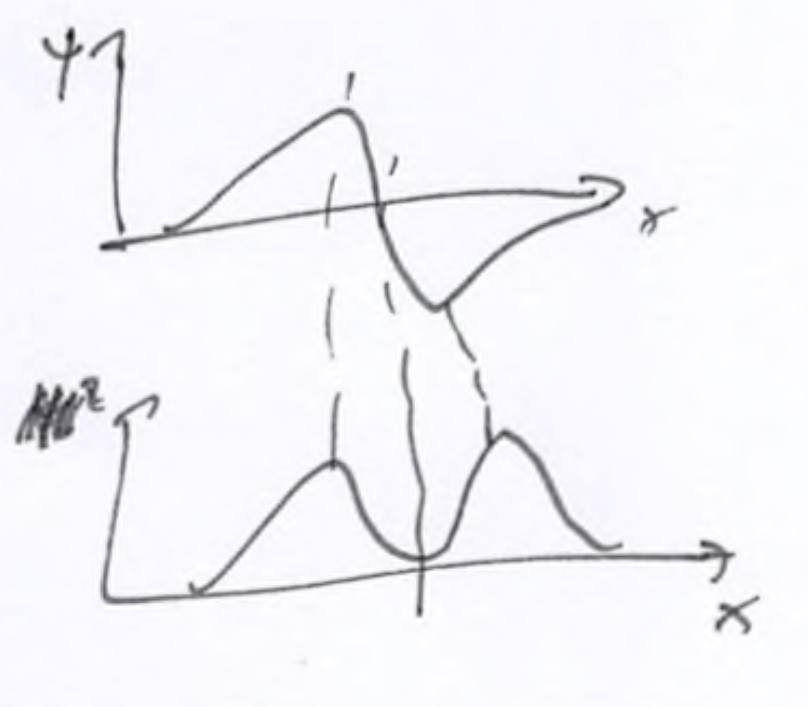
\includegraphics[width=\textwidth]{\currfiledir sketch/wavefunction.png}
    \caption{Eine Wellenfunktion $\Psi(x)$ könenn wir nicht direkt messen, sondern nur ihr Betragsquadrat $|\Psi(x)|^2$.}
\end{marginfigure}



\subsection{Normierung}

Wie bei den Dartpfeilen muss die Summe aller sich gegenseitig ausschließenden Wahrscheinlichkeiten eins ergeben. Irgendwo muss das Elektron detektiert werden, es kann nicht verschwinden. Für diskrete Bereiche $A$, $B$, $C$ usw. schreibt man dies als
\begin{equation}
    \sum_{j = A, B, C, \dots} P_j = 1 \quad .
\end{equation}
Mit der Wahrscheinlichkeitsdichte wird die Summe ein Integral, d.h.
\begin{equation}
    \int_{-\infty}^{+\infty} P(x) dx = 1 \quad .
\end{equation}
Dies hat Konsequenzen für die Wellenfunktion $\Psi(x)$. Da $P(x) = |\Psi(x)|^2$, muss also 
\begin{equation}
    \int_{-\infty}^{+\infty} |\Psi(x)|^2 dx = 1 \quad .
\end{equation}
Dies wird Normierungsbedingung genannt, oder eine Wellenfunktion ist normiert, wenn sie diese Bedingung erfüllt. Noch einmal: Wir können nur etwas über das Quadrat der Wellenfunktion sagen, aber nichts über die Wellenfunktion selbst, und damit auch nichts über ein Integral der Wellenfunktion selbst.

\begin{questions}
    \item Welche Einheit hat eine Wellenfunktion $\Psi(x)$ ?
\end{questions}


\section{Korrespondenzprinzip}
An verschiedenen Stellen ist uns der Welle-Teilchen-Dualismus begegnet. Objekte auf der atomaren Skala können nicht mehr nur als Welle oder nur als Teilchen beschrieben werden, sondern sind beides oder nichts von beidem. Unsere Bilder sind zu schwach, um diese Objekte zu beschreiben. Es hat sich aber gezeigt, dass man den Übergang von der mikroskopischen zur makroskopischen Welt nutzen kann, um die Konsistenz der mikroskopischen Beschreibung zu überprüfen. 

Wir fragen uns also, ob das mikroskopische Modell noch funktioniert, wenn wir alles noch größer machen. Bei den Photonen am Doppelspalt zum Beispiel, indem wir die Anzahl der Photonen pro Fläche stark erhöhen, oder beim Teilchen im Kasten, indem wir die Quantenzahl $n$ sehr groß machen. Das \emph{Korrespondenzprinzip} besagt, dass das mikroskopische Modell für große Quantenzahlen in das entsprechende makroskopische Modell übergehen muss. Bei großen Quantenzahlen ist der Effekt der Quantisierung nicht mehr wahrnehmbar, der Unterschied zwischen benachbarten Quantenzahlen ist klein. Dies haben wir in den letzten Abschnitten ausgenutzt, um die Wellenfunktion der Photonen zu konstruieren: für große Photonenzahlen muss alles in die klassische Elektrodynamik übergehen.



\section{Wellenpakete}

\begin{marginfigure}
    \inputtikz{\currfiledir wavepaket}
    \caption{Skizze eines Wellenpakets}
    \label{fig:3_wellenpaket}
\end{marginfigure}

Welle und Teilchen sind zwei klassische Konzepte, die sich gegenseitig ausschließen. Keines von beiden kann allein das Doppelspaltexperiment beschreiben und den Welle-Teilchen-Dualismus auflösen. Klassische Wellenpakete zeigen jedoch viele Eigenschaften, die wir auch auf der atomaren Skala finden. Sie können deshalb als Modell dienen.

Betrachten wir ein Wellenpaket, wie es in Abbildung~\ref{fig:3_wellenpaket} skizziert ist. Im Gegensatz zu einer Sinuswelle ist das Wellenpaket räumlich und zeitlich begrenzt. Dadurch ähnelt es einem Teilchen. Gleichzeitig hat ein Wellenpaket aber auch eine Wellenlänge und schwingt wie eine Welle in Raum und Zeit. Aber auch Wellenpakete sind kein ideales Modell. Letztlich beschreibt nur die Quantenmechanik Objekte auf atomarer Skala korrekt.

Überlagern sich zwei Sinuswellen mit den Frequenzen $f_1$ und $f_2$, so entsteht eine Schwebung (engl beating). Die Amplitude der Gesamtwelle ändert sich periodisch mit der Schwebungsfrequenz
\begin{equation}
    f_{beat} = | f_1 - f_2 | = \frac{1}{T_{beat}} \quad . \label{eq:3_tbeat}
\end{equation}
Es entsteht also eine Abfolge von Wellenpaketen mit dem Abstand $T_{beat}$. Nennen wir die Differenz der beiden Frequenzen $\Delta f$ und die Länge der Wellenpakete $\Delta t$ (also ihren Abstand $T_{beat}$, also $T_{beat} = \Delta t$), so können wir Gl. \ref{eq:3_tbeat} schreiben als
\begin{equation}
    \Delta t \, \Delta f = 1 \quad .
\end{equation}
Das ist zunächst trivial, aber es ist ein Vorbote von etwas Größerem. Wenn sich die beiden Frequenzen annähern, werden die Wellenpakete länger.


\begin{marginfigure}
   \inputtikz{\currfiledir wavepaket_synthesis}
    \caption{Synthese eines Wellenpakets}
    \label{fig:3_Synthese}
\end{marginfigure}


Um nicht einen Zug von Wellenpaketen, sondern ein einziges Paket zu erhalten, müssen viele Sinuswellen überlagert werden. Zum Zeitpunkt $t=0$ überlagern sich alle konstruktiv (siehe Skizze~\ref{fig:3_Synthese}), zu allen anderen Zeitpunkten jedoch mehr oder weniger destruktiv. Insbesondere gibt es für große Zeiten zu jeder Welle immer eine andere, die diese gerade auslöscht. Der Zusammenhang zwischen den Frequenzkomponenten und dem zeitlichen Verlauf wird durch die Fourier-Transformation hergestellt. Eine Eigenschaft der Fourier-Transformation ist die Pulsdauer-Bandbreiten-Grenze
\begin{equation}
    \Delta t \, \Delta f \approx 1 \quad .
\end{equation}
Der genaue Wert der Konstanten auf der rechten Seite hängt von der zeitlichen Form des Wellenpakets ab und auch davon, wie genau man die Breiten $\Delta t$ und $\Delta f$ definiert. Auf diese Details soll hier nicht eingegangen werden. Ich verstecke alles in 'ungefähr eins'. Die Bedeutung ist unabhängig von diesen Details: Ein Wellenpaket, das aus der Superposition verschiedener Sinuswellen gebildet wird, kann nicht beliebig kurz sein. Es hat eine minimale Länge $\Delta t$, die sich aus seiner Breite im Frequenzraum $\Delta f$ ergibt. Dies ist schon eine Eigenschaft der Fourier-Transformation und gilt daher auch in der klassischen Physik.


\begin{questions}
    \item Erzeugen Sie in der Simualtion\phet{Fourier_Making_Waves} Wellenpakete.
\end{questions}

\subsection{Bandbreite}

Die Pulsdauer-Bandbreitenbegrenzung der Fourier-Transformation hat verschiedene technische Konsequenzen. Immer dann, wenn die Breite im Frequenzbereich begrenzt ist, ist auch die zeitliche Dauer nach unten begrenzt. Ein Beispiel hierfür sind kurze Laserpulse. Um einen Laserpuls der Länge $\Delta t = 100 fs = 100 \cdot 10^{-15}$s zu erzeugen, benötigt man ein Spektrum, das mindestens 
\begin{equation}
    \Delta f = \frac{1}{100 fs} = 10 \cdot 10^{12} Hz = 10 THz
\end{equation}
breit ist. Bei einer Zentralwellenlänge von 800~nm entspricht dies einer Breite von etwa 20~nm.


\subsection{Unschärfe}

Die Breiten $\Delta t$ und $\Delta f$ können auch als \emph{Unschärfe} verstanden werden. Bei einem Wellenpaket der Zeitlänge $\Delta t$ können wir nicht mehr eindeutig sagen, wann es am Detektor eintrifft. Ist die Ankunftszeit der Anfang des Pakets oder das Ende oder das Maximum? Ebenso können wir nicht mehr eindeutig sagen, welche Frequenz und damit welche Wellenlänge es hat, da verschiedene Sinuswellen zum Wellenpaket beitragen. Dies ist eine grundsätzliche Eigenschaft von Wellenpaketen und hat nichts mit experimentellen Unzulänglichkeiten zu tun.

Diese beiden Unschärfen sind miteinander verknüpft. Wenn wir ein Wellenpaket erzeugen wollen, das zeitlich sehr gut definiert ist, also eine kleine zeitliche Unschärfe $\Delta t$ hat, dann verlangt die Pulsdauer-Bandbreiten-Grenze, dass die Frequenzunschärfe $\Delta f$ besonders groß ist. Und umgekehrt: Wenn die Frequenz in einem Wellenpaket sehr genau bekannt sein soll, $\Delta f$ also klein sein soll, dann kann man nur sehr ungenau angeben, wann dieses Wellenpaket eintrifft.

Technisch ist 
\begin{equation}
    \Delta t \, \Delta f \approx 1
\end{equation}
eine untere Grenze. Aufgrund von Rauschen oder anderen technischen Faktoren kann die zeitliche Dauer oder die Bandbreite noch größer sein. Dieses Produkt aus Pulsdauer und Bandbreite definiert die Grenze des Wissens, das über ein beliebiges Wellenpaket gewonnen werden kann.


\section{Die Heisenbergsche Unschärfe-Relation}

Wir wollen nun ein Teilchen durch ein Wellenpaket beschreiben. Das Teilchen mit der Masse $m$ bewegt sich mit der Geschwindigkeit $v_x$ entlang der Achse $x$. Seine de Broglie-Wellenlänge ist $\lambda = h / p_x$ mit $p_x = m v_x$ der x-Komponente des Impulses. Die Periodendauer des Wellenpakets sei $\Delta t$. Dann ist die räumliche Ausdehnung $\Delta x$.
\begin{equation}
    \Delta x = v_x \Delta t = \frac{p_x}{m} \, \Delta t \quad .
\end{equation}

Die Frequenz $\nu$ der Materiewelle des Teilchens ergibt sich aus dessen de Broglie-Wellenlänge via\sidenote{hier ist Phasen- gleich Gruppengeschwindigkeit}
\begin{equation}
    \nu \lambda = v
\end{equation}
also 
\begin{equation}
    \nu = \frac{v}{\lambda } = \frac{p_x / m}{h / p_x} = \frac{p_x^2}{h m} \quad .
\end{equation}
Durch Ableitung finden wir
\begin{equation}
    \Delta \nu = \frac{2 p_x}{h m} \, \Delta p_x \quad .
\end{equation}
Wenn wir all dies in die Gleichung für Pulsdauer und Bandbreite einsetzen (und die Frequenzen auf der atomaren Skala als $\nu$ schreiben), dann erhalten wir
\begin{equation}
    \Delta t \Delta \nu = \frac{m}{p_x} \Delta x \, \, \frac{2 p_x}{h m} \, \Delta p_x = \frac{2}{h} \, \Delta x \, \Delta p_x   \quad .
\end{equation}
Die Pulsdauer-Bandbreiten-Grenze ist ja eine untere Grenze. Darum schreibe ich das $\approx$ jetzt als $\ge$ und wir erhalten
\begin{equation}
    \Delta x \, \Delta p_x  \ge  \frac{h}{2} \quad .
\end{equation}
Dies ist die \emph{Heisenbergsche Unschärferelation}, in dieser Form auch Orts-Impuls-Unschärfe genannt. Wie oben hängt die rechte Seite der Gleichung von der genauen Definition der beiden Breiten $\Delta x$ und $\Delta p_x$ ab. Aber auch hier sind die Details nicht so wichtig, solange ein $h$ auftaucht.

\paragraph*{Was bedeutet das?} Die Heisenbergsche Unschärferelation beschreibt die Grenze unseres Wissens über ein quantenmechanisches Teilchen. Wir können nicht gleichzeitig den Ort und den Impuls (oder die Geschwindigkeit) beliebig genau kennen. Je genauer wir den Ort kennen wollen, desto ungenauer muss unser Wissen über den Impuls sein und umgekehrt.

Messunsicherheiten sind ein Charakteristikum der klassischen Physik. Jede Messung ist mit einer Unsicherheit behaftet. In der klassischen Physik ist dies jedoch ein rein technisches Problem. Mit etwas mehr Aufwand könnte man die Unsicherheit reduzieren. Außerdem sind zwei Messungen, z.B. Ort und Geschwindigkeit, voneinander unabhängig, und wir könnten beide Unsicherheiten getrennt voneinander behandeln.

Die Heisenbergsche Unschärferelation besagt, dass dies in der atomaren Welt nicht der Fall ist. Es handelt sich nicht mehr um ein technisches Problem, sondern um eine grundsätzliche Grenze unseres Wissens. Wie auch immer wir es technisch machen, Ort und Impuls können nicht beliebig genau bestimmt werden. In dieser Hinsicht sind atomare Teilchen Wellenpaketen ähnlich.

\paragraph*{Nebenbemerkung} Wenn Sie eine Vorlesung über Quantenmechanik besucht haben, werden Sie gesehen haben, dass die Heisenbergsche Unschärferelation mit den Operatoren $\hat{A}$, $\hat{B}$ geschrieben wird als\footcite{Nolting-QM} 
\begin{equation}
    \Delta A \, \Delta B \ge \frac{1}{2} \left|   \braket{ [\hat{A}, \hat{B}]  } \right|
\end{equation}
wobei die eckige Klammer $[ \cdots]$ den Kommutator darstellt\sidenote{$[\hat{A}, \hat{B}] = \hat{A} \hat{B} - \hat{B} \hat{A}$} und die spitze Klammer $\braket{\cdots}$ den Erwartungswert bezeichnet. Auf diese Weise erhält man die oben hergeleitet Orts-Impuls-Unschärfe.

Die Pulsdauer-Bandbreiten-Unschärfe, oder durch Multiplikation mit $h$ die Energie-Zeit-Unschärfe
\begin{equation}
    \Delta E \, \Delta t \ge h
\end{equation}
ist aber eigentlich keine Heisenbergsche Unschärferelation im engeren Sinne, weil es in der Quantenmechanik keinen Zeitoperator gibt. Sie ist 'nur' eine Eigenschaft der Fourier-Transformation. Diese Unterscheidung wird aber nicht oft geamcht.


\begin{questions}
    \item \emph{Quantenradierer} sind eine Klasse von Doppelspaltexperimenten mit Quanten, bei denen eigentlich der Weg des Photons durch den einen oder anderen Spalt gemessen wird, diese Information dann aber wieder 'ausradiert' wird. Eine (alte) populärwissenschaftliche Darstellung ist \cite{WT_dualismus}, neuere sind \cite{heise_quantenradierer} und \cite{Hossenfelder_quantenradierer}. Ist das jetzt ein Paradoxon, oder nicht?
\end{questions}



\section{Zusammenfassung}

\textit{Schreiben Sie hier ihre persönliche Zusammenfassung des Kapitels auf. Konzentrieren Sie sich auf die wichtigsten Aspekte.}

\vspace*{10cm}


%--------------------


\printbibliography[segment=\therefsegment,heading=subbibliography]
